\section{Desenvolvimento}
Nesta seção vamos entrar mais a fundo no processo de desenvolvimento dos analisadores usando as ferramentas geradoras desenvolvidas em Java. Os códigos passados para os geradores estão descritos na próxima seção.

\subsection{Analisador Léxico}
A criação do analisador léxico foi feita usando a ferramenta geradora \textbf{JFlex}\cite{klein_2017}. Diversas outras existem, tanto escritas em Java, como a \textbf{JLex}, ou em C, como a \textbf{Lex} e a \textbf{Flex}. No entanto, nossa escolha foi baseada no fato de a JFlex dar muita maleabilidade ao código e ainda estar sob constante desenvolvimento. Atualmente ela está na versão 1.6.1. 

O arquivo \texttt{Lexer.flex} contém as instruções para modelagem do analisador léxico. Nele são descritas as expressões regulares e símbolos a serem procurados e extraídos de um dado código fonte. Para tal processo, o analisador é formado por um autômato finito determinístico(AFD). Inicialmente, um autômato finito não-determinístico(AFN) é gerado, este é convertido em um AFD que é então minimizado. Um exemplo de saída criada nesse processo pode ser visto na figura 2.

\begin{figure}[h]	
 \centering
  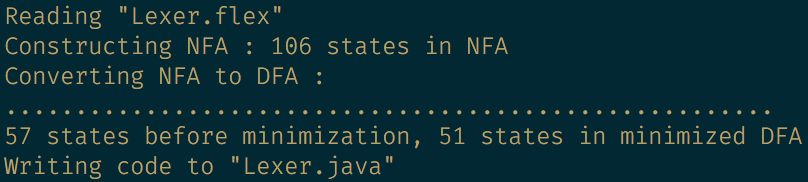
\includegraphics[width=10cm,keepaspectratio]{images/lexer.png}
 \caption{Saída gerada na criação do analisador léxico pelo JFlex.}
\end{figure}

Para executar o JFlex é necessária a execução da seguinte sequência via linha de comando:

\begin{Verbatim}[frame=single]
java -jar jflex-1.6.1.jar Lexer.flex
\end{Verbatim}

Com a adição da opção \texttt{-{}-dot} ainda é possível obter as máquinas de estados em todas as suas etapas(AFN, AFD, AFD minimizada) no formato \texttt{.dot}. Assim, através do uso da biblioteca \texttt{graphviz}, é possível converter os arquivos \texttt{.dot} para \texttt{.png} com o seguinte comando:

\begin{Verbatim}[frame=single]
dot -Tpng afd.dot afd.png
\end{Verbatim}

Nenhum autômato finito foi apresentado aqui devido ao tamanho impraticável de suas representações gráficas.

\subsection{Analisador Sintático}
A criação do analisador sintático LALR for feita usando o gerador \textbf{CUP}\cite{cup_2017}, que atualmente está em sua versão 0.11b e é mantido pela \textit{Technical University of Munich}. O CUP tem integração direta com o JFlex, o que simplifica em muito o processo. O arquivo \texttt{Parser.cup} contém as instruções para construção do analisador, como a descrição dos terminais, não-terminais e as regas da gramática. Os símbolos definidos na fase de análise léxica são fundamentais aqui. 

A saída do gerador nos fornece alguns dados sobre as dimensões do parser e sua integridade ao longo do processo, como pode ser visto na figura 3. Para executarmos o CUP, é necessário o seguinte comando:

\begin{Verbatim}[frame=single]
java -jar java-cup-11b.jar -interface -parser Parser Parser.cup
\end{Verbatim}

\begin{figure}[h]	
 \centering
  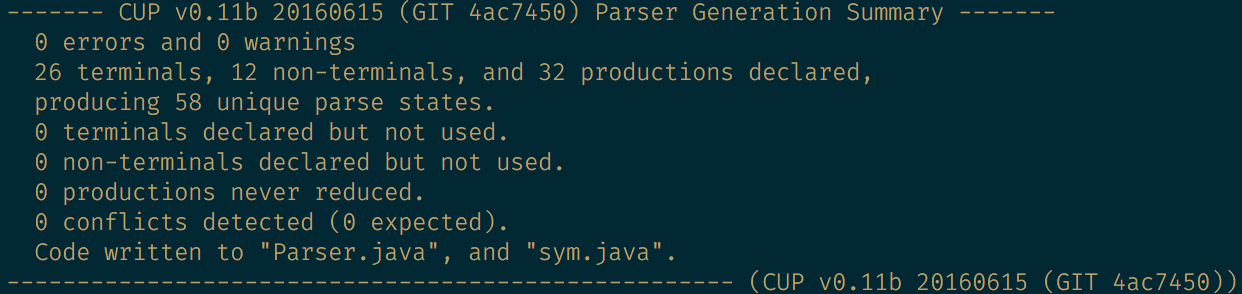
\includegraphics[width=10cm,keepaspectratio]{images/parser.png}
 \caption{Saída gerada na criação do analisador sintático pelo CUP.}
\end{figure}

Houve um conflito do tipo \texttt{shift-reduce} na gramática com relação  a regra do \texttt{if} sozinho ou do \texttt{if-else}, acusado pelo CUP com a saída demonstrada na figura 4. Esse conflito foi resolvido ao darmos precedência à esquerda para o símbolo ELSE.

\begin{figure}[h]	
 \centering
  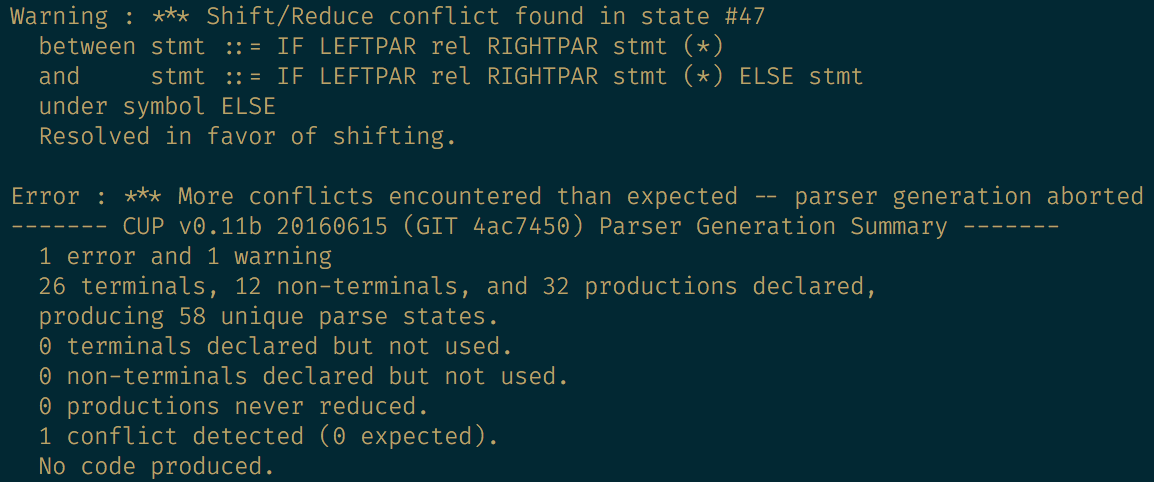
\includegraphics[width=10cm,keepaspectratio]{images/shift-reduce.png}
 \caption{Saída acusando conflito shift-reduce.}
\end{figure}

\subsection{Integração de Analisadores}

Para que ambos analisadores funcionem em conjunto, é necessário a execução de uma biblioteca de \textit{runtime} do CUP. Essa execução é feita da seguinte forma:

\begin{Verbatim}[frame=single]
javac -cp java-cup-11b-runtime.jar:. *.java
\end{Verbatim}

Agora o arquivo \texttt{Parser.class} pode ser chamado por linha de comando para execuções das funções de análise, como será demonstrado na seção 4.